\documentclass[11pt]{article}
%%%%%%%%%%%%%%%%%%%%%%%%%%%%%%%%%%%%%%%%%

\usepackage{amscd}
\usepackage{amsmath}
\usepackage{amssymb}
\usepackage{amsthm}


\usepackage{epsfig}
\usepackage{verbatim}
\usepackage{graphicx}
\usepackage{amsthm}
\usepackage{multirow}
%\usepackage{hyperref}
\pagestyle{empty}
\usepackage{color}
\usepackage[left=3cm,top=2.5cm,right=3cm,bottom=3cm]{geometry} % Document margins
%\usepackage[all,dvips]{xy}


\begin{comment}  

This LaTeX document is a template to be used by Bates mathematics rising seniors to create a thesis proposal. 

As a guide, the document is already filled out to represent a fictitious proposal, and all you need to do is modify the entries below to represent your own proposal.

A PDF version of the fictitious proposal is available on the department's FAQ and Policies pages, at
http://abacus.bates.edu/acad/depts/math/faq.html
and
http://abacus.bates.edu/acad/depts/math/policies.html
respectively.

Once you have finished your proposal, export it to a PDF file. Give the file a USEFUL name, for example, RiemannThesisProposal.PDF. Email the PDF file to Clementine Brasier, the 
Academic Administrative Assistant for Hathorn Hall, at cbrasier\@bates.edu

This LaTex document was created Feb/Mar 2010 by Adriana Salerno and updated Feb 2012 by Meredith Greer

\end{comment}


%%%%%%%%%%%%%%%%%%%%%%%%%%%%%%%%%%%%%%%%%

\begin{document}
	\begin{titlepage}
		\centering
		
\includegraphics[width=0.15\textwidth]{NU_logo.png}\par\vspace{1cm}
		{\scshape\LARGE Northeastern University \par}
		\vspace{1cm}
		{\scshape\Large NLP Project Report\par}
		\vspace{1.5cm}
		{\huge\bfseries Plagiarism Detection Using FP-Growth Algorithm\par}
		\vspace{2cm}
		{\Large\itshape Varun Nandu\par}
		{\Large\itshape (nandu.v@husky.neu.edu) \par}
		{\Large\itshape Suraj Nair\par}
		{\Large\itshape (nair.sur@husky.neu.edu) \par}
		\vfill
		Supervised by\par
		Dr. Lu Wang  \textsc{}
		
		\vfill
		
		% Bottom of the page
		{\large \today\par}
	\end{titlepage}
	
	\section{Introduction and Related Work}
	
	Plagiarism is the "wrongful appropriation" and "stealing and publication" of another author's "language, thoughts, ideas, or expressions" and the representation of them as one's own original work.
Plagiarism is considered academic dishonesty and a breach of journalistic ethics. This is a growing problem in todays times in educational institutions. Thus in order to protect one's academic integrity plagiarism detection has gained a lot of importance these days. Previously, works such as Plagiarism Detection Using the Levenshtein Distance and Smith-Waterman Algorithm \cite{pdld} where the Levenshtein distance between two strings is given by the minimum number of operations, and that needed to transform one string into the other, where an operation is an insertion, deletion, or substitution of a single character is seen.  We also came across Intrinsic Plagiarism Detection Using Character n-gram \cite{ngram}. This algorithm attempts to quantify the style variation within a document using character n-gram profiles and a style change function based on an appropriate dissimilarity measure originally proposed for author identification. In this project, we used some basic idea from the above methods and implemented a plagiarism detection on a completely different concept. We used unsupervised machine learning algorithm called using Frequent Pattern (FP) Growth Algorithm.

	The FP-Growth Algorithm, proposed by Han \cite{han1}, is an efficient and scalable method for mining the complete set of frequent patterns by pattern fragment growth, using an extended prefix-tree structure for storing compressed and crucial information about frequent patterns named frequent-pattern tree (FP-tree). FP-Growth algorithm is normally used to find frequent item-sets given a number of transactions. In natural language processing, we can model our text data into vectors using word vector vector representation techniques. Many word vector representation techniques have been developed in recent times. We will use GloVe \cite{glove} to represent our textual data in form of vectors. Thus we get a vector representing each unique word in our data.
	
	For getting similar words in context and meaning, many methods have been used like Brown Clustering Algorithm \cite{brown} or Word2Vec\cite{w2v2}. However in our project, we use K-means \cite{kmeans} Clustering Algorithm because of its features like completeness, exclusivity and fast execution. In our project, clusters of similar words are created. Then a vector for each sentence is built based on those clusters. If the two words belong to the same cluster then, the same cluster number is applied to both the words in the vector. After that a vector for each text document is created based on sentence vectors. If two sentence vectors are similar, then we assign a unique number to those sentences. Thus we get a vector for each document which we can use as item-sets in the FP-Growth Algorithm and the number of documents will be our transactions. Once we get frequent item sets we know which documents are plagiarised from each other.
	
	\bigskip
	
	
	\section{Dataset and Features} 
		\subsection{Dataset}
		 In this study, the freely available Clough-Stevenson corpus \cite{corpus} was applied. The corpus consists of answers to five short questions on a variety of topics in Computer Science field. The five short questions are:
1. What is inheritance in object oriented programming?
2. Explain the PageRank algorithm that is used by the Google search engine. 3. Explain the Vector Space Model that is used for Information Retrieval.
4. Explain Bayes Theorem from probability theory.
5. What is dynamic programming?

		
		Each question has 19 students answers and 1 wikipedia answer. We are also given which answers are plagiarised. There are four different types of answers. They are cut, light, non and heavy. Cut refers to answers that are cut, copy, pasted from wikipedia answer. Heavy refers to answers that are heavily copied from wikipedia answers, light refers to answers which are slightly copied from wikipedia answers with extreme changes to the structure of answers. Non refers to non plagiarised work. We can view this in the table given below.
		\begin{table}[htb]
			\caption{Dataset statistics} 
			\label{tab:1}
			\begin{center}
				\begin{tabular}{|c|c|}
					\hline
					Number of questions & 5 \\
					\hline
					Number of answers per question & 20 \\
					\hline
					Number of Non or lightly plagiarised answers & 57 \\
					\hline
					Number of Heavily plagiarised answers & 19 \\
					\hline
					Mean no of words per answer & 216 \\
					\hline
				\end{tabular}
				
			\end{center}
		\end{table}
		
		Thus the input for our system is various documents which contain student answers for various questions. The output is the list of students that have plagiarised work for each question. 
		\subsection{Pre-Processing and Setup}
	For pre-processing we have to make sure that all the words are lower cased with all the punctuations removed. We use the NLTK sentence tokeniser to get list of sentences so that we know where does each sentence begin and end. There are various latin words in our answers as well so we use "latin1" encoding for reading the text. After preprocessing the text we needed a way to cluster similar words. Since, we were using K-means clustering which is a distance based clustering method, we needed each unique word in our corpus to have a numerical value. Thus, for creating vector word embeddings, we used a method called GloVe.
	GloVe is an unsupervised learning algorithm for obtaining vector representations for words. Training is performed on aggregated global word-word co-occurrence statistics from a corpus, and the resulting representations showcase interesting linear substructures of the word vector space.
	The statistics of word occurrences in a corpus is the primary source of information available to all unsupervised methods for learning word representations, and although many such methods now exist, the question still remains as to how meaning is generated from these statistics, and how the resulting
word vectors might represent that meaning.
The GloVe model is trained on the non-zero entries of a global word-word co-occurrence matrix, which tabulates how frequently words co-occur with one another in a given corpus. Populating this matrix requires a single pass through the entire corpus to collect the statistics. For large corpora, this pass can be computationally expensive, but it is a one-time up-front cost. Subsequent training iterations are much faster because the number of non-zero matrix entries is typically much smaller than the total number of words in the corpus. GloVe is essentially a log-bilinear model with a weighted least-squares objective. The main intuition underlying the model is the simple observation that ratios of word-word co-occurrence probabilities have the potential for encoding some form of meaning. 

	After performing GloVe on our preprocessed data we get vector of each unique word in our corpus. We can use this representation for clustering and further processing.

				
		\section{Processing Methods}
		
		\subsection{K-means Clustering}
		K-means clustering is a type of unsupervised learning, which is used when we have unlabelled data (i.e., data without defined categories or groups). The goal of this algorithm is to find groups in the data, with the number of groups represented by the variable K. The algorithm works iteratively to assign each data point to one of K groups based on the features that are provided. Data points are clustered based on feature similarity. The results of the K-means clustering algorithm are:

	\begin{description}
\item	[$\bullet$ ]The centroids of the K clusters, which can be used to label new data.

	\item	[$\bullet$ ]Each data point is assigned to a single cluster.
	\end{description}
	
Rather than defining groups before looking at the data, clustering allows you to find and analyze the groups that have formed organically. The "Choosing K" section below describes how the number of groups can be determined.�Each centroid of a cluster is a collection of feature values which define the resulting groups. Examining the centroid feature weights can be used to qualitatively interpret what kind of group each cluster represents. 
		
		\begin{figure}
			\centering
			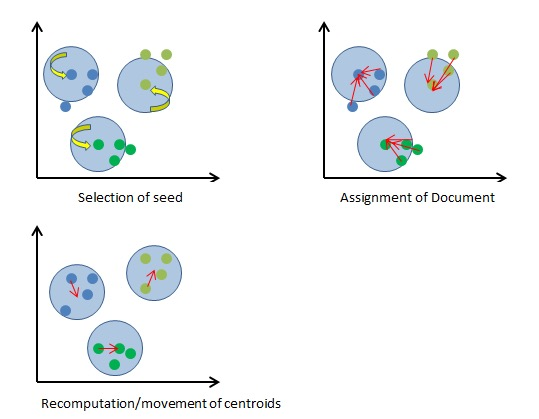
\includegraphics{k-means-process.jpeg}
			\caption{K-means clustering $(Image Courtesy: Data Science world \cite{kmeans})$. }
			\label{fig:cnn}
		\end{figure}
		
\subsubsection {Algorithm}

The k-means clustering algorithm uses iterative refinement to produce a final result. The algorithm inputs are the number of clusters 'k' and the data set. The data set is a collection of features for each data point. The algorithms starts with initial estimates for the 'k' centroids, which can either be randomly generated or randomly selected from the data set. The algorithm then iterates between two steps:

1. Data assigment step:

Each centroid defines one of the clusters. In this step, each data point is assigned to its nearest centroid, based on the squared Euclidean distance. More formally, if ci is the collection of centroids in set C, then each data point x is assigned to a cluster based on

$$\underset{c_i \in C}{\arg\min} \; dist(c_i,x)^2$$

where dist( � ) is the standard (L2) Euclidean distance. Let the set of data point assignments for each ith cluster centroid be Si.

2. Centroid update step:

In this step, the centroids are recomputed. This is done by taking the mean of all data points assigned to that centroid's cluster.

$$c_i=\frac{1}{|S_i|}\sum_{x_i \in S_i x_i}$$

The algorithm iterates between steps one and two until a stopping criteria is met (i.e., no data points change clusters, the sum of the distances is minimized, or some maximum number of iterations is reached).

This algorithm is guaranteed to converge to a result. The result may be a local optimum (i.e. not necessarily the best possible outcome), meaning that assessing more than one run of the algorithm with randomized starting centroids may give a better outcome.

\subsubsection {Implementation}

K-means clustering algorithm is that it is not guaranteed to find the most optimal cluster arrangement, if you pick the wrong starting points. One method for overcoming this is to run the algorithm a number of times with different randomly selected starting points, and then pick the solution that has the lowest total squared Euclidean distance. This approach is used in the scikit-learn package, defaulting to 10 separate repetitions. Scikit-learn implementation of K-Means returns an object that indicates the cluster to which each input vector belongs. Thus after performing K-means clustering, we get similar word clusters. Now, we need to apply FP-growth Algorithm to find frequent item sets. But in order to do that, we first need to represent our data in the form of transactions of various item-sets. In order to do that we created our own vector representation explained below.

\subsection{Vector Representation}
From the obtained clusters and its respective labels from K-means clustering algorithm, we now use these clusters to convert our data in each documents to vectors. For this, we do the following.
\begin{description}
\item	[$\bullet$ ] Determine the cluster label for each of the word in sentences and substitute the word with its respective cluster label. 
\item	[$\bullet$ ] From the above step, we merge all the words and form sentence vectors. 
\item	[$\bullet$ ] From these sentence vector, we form answer vector by assigning a unique number if two sentence vectors are different. If two sentence vectors are same we assign each of them the same number. 
\end{description}

Thus we get a vector for each answer. This vector can be viewed as an item-set and each answer can be viewed as a transaction.Thus we get a list of transactions which contain item-sets. We can feed this into FP-Growth Algorithm to get frequent item sets.

\subsection{FP-growth algorithm}
The FP-growth algorithm is currently one of the fastest approaches to frequent item set mining. One of the currently fastest and most popular algorithms for frequent item set mining is the FP-growth algorithm \cite{fpgrowth}. It is based on a prefix tree representation of the given database of transactions (called an FP-tree), which can save considerable amounts of memory for storing the transactions. The basic idea of the FP-growth algorithm can be described as a recursive elimination scheme: in a preprocessing step delete all items from the transactions that are not frequent individually, i.e., do not appear in a user-specified minimum number of transactions. Then select all transactions that contain the least frequent item (least frequent among those that are frequent) and delete this item from them. Recurse to process the obtained reduced (also known as projected) database, remembering that the item sets found in the recursion share the deleted item as a prefix. On return, remove the processed item also from the database of all transactions and start over, i.e., process the second frequent item etc. In these processing steps the prefix tree, which is enhanced by links between the branches, is exploited to quickly find the transactions containing a given item and also to remove this item from the transactions after it has been processed.

Thus after performing FP-Growth Algorithm we get frequent item sets. In our context we get frequent sentences which are plagiarised. We can find which sentences are plagiarised by just looking at the transactions which in our case are student answers. Now it is important to know that we need to consider only three or more frequent item-sets meaning only three or more plagiarised sentences. This is because most of the students can have one one or two similar sentences like "This is called Inheritance". We cannot penalise students for that.

\section{Results}	
As, described in Section 2, Each question has 19 students answers and 1 wikipedia answer. We calculated all the ground truth for our data. When we ran our method on the dataset we got the following results:

	\begin{table} [htb]
			\caption{Evaluation Metrics} 
			\label{tab:1}
			\begin{center}
				\begin{tabular}{|c|c|}
					\hline
					Precision & 90\% \\
					\hline
					Accuracy & 94.03\% \\
					\hline
					Recall & 52.33\% \\
					\hline
					F1-score & 66.18\% \\
					\hline
				\end{tabular}
			\end{center}
	\end{table}
The table below shows the plagiarised task and student names obtained form our algorithm. 

\begin{table}  [htb]
			\caption{Plagiarism detection} 
			\label{tab:2}
			\begin{center}
				\begin{tabular}{|c|c|}
					\hline
					taske & orig, g0pE, g2pB, g1pB \\
					\hline
					taska & g0pE, g3pC, g2pC, g4pC, orig \\
					\hline
					taskd & g2pA, g4pC, g3pA \\
					\hline
					
				\end{tabular}
				
			\end{center}
		\end{table}
	
	Thus we got some decent results. Although, not absolutely great, the results were better than the previous methods we discussed. For example the Plagiarism Detection using n-gram method had a precision of 47\%. Our precision as can be seen above is much higher than that.  
	\section{Future work}
	Many methods have been proposed to detect and stop plagiarism. But, still there are many questions which are to be answered. Natural Language Processing has greater possibilities of providing a sound and concrete mechanism which is capable of detecting plagiarism in any document. In this report we have tried to show finding plagiarism��using FP-growth with its advantages. We have developed a system based on principles of vector representations. As an extension to this work, we can include vector representations using other techniques such as word2vec.  Another future work is to change the domain from documents to programming. In programming, we would need stricter noise removal as well as the support count of FP-growth algorithm will increase.
	
	
	\begin{thebibliography}{99}
		% NOTE: change the "9" above to "99" if you have MORE THAN 10 references.
		
		\bibitem{han1} J. Han, H. Pei, and Y. Yin. Mining Frequent Patterns without Candidate Generation. In: Proc. Conf. on the Management of Data (SIGMOD?00, Dallas, TX). ACM Press, New York, NY, USA 2000
		\bibitem{pdld} http://ieeexplore.ieee.org/stamp/stamp.jsp?arnumber=4603758
		\bibitem{ngram} http://citeseerx.ist.psu.edu/viewdoc/summary
		\bibitem{brown} Percy Liang (2005). Semi-Supervised Learning for Natural Language (PDF) (M. Eng.). MIT. pp. 44?52
		
		\bibitem{w2v2} Tomas Mikolov, Ilya Sutskever, Kai Chen, Greg Corrado and Jeffrey Dean. \textit{Distributed Representations of Words and Phrases and their Compositionality}, In NIPS, 2013
		
		\bibitem{kmeans} https://en.wikipedia.org/wiki/K-meansclustering
		
		\bibitem{corpus} P. Clough and M. Stevenson. ?Developing a Corpus of Plagiarized Short Answers, Language Resources and Evaluation: Special Issue on Plagiarism and Authorship Analysis, In Press.? Internet: http://ir.shef.ac.uk/cloughie/resources/plagiarismcorpus.html/Download, Sep. 10, 2009 [Oct. 12, 2011].
		
				
		\bibitem{glove} Jeffrey Pennington and Richard Socher and Christopher D. Manning. \textit{GloVe: Global Vectors for Word Representation}, p 1532 - 1543,  
		EMNLP 2015
		
		\bibitem{glovecode} https://github.com/stanfordnlp/GloVe
		
		\bibitem{kmeans} https://www.datascience.com/blog/k-means-clustering
		\bibitem{kmeansexp} http://douglasduhaime.com/posts/clustering-semantic-vectors.html
		
		\bibitem {fpgrowth} https://www.researchgate.net/profile/Christian-Borgelt/publication/234774858-keeping-things-simple-Finding-frequent-item-sets-by-recursive-elimination/links/00b7d514b21cd06b09000000.pdf
		
	\end{thebibliography}
	%%%%%%%%%%%%%%%%%%%%%%%%%%%%%%%%%%%%%%%%%

	
\end{document} 
